\documentclass{jsarticle}
\usepackage[dvipdfmx]{graphicx}
\usepackage{listings}
\usepackage{afterpage}
\begin{document}
\title{マイコン基礎及び演習}
\author{13EC060 武澤 裕介}
\maketitle
\begin{abstract}
AVRマイコンによるLED及びモータの同時制御方法について述べ、考察し改善点などを指摘する。
\end{abstract}
\section{設計仕様}
設計仕様は以下である。
\begin{itemize}
\item 停止状態:LED が 5 秒毎に点滅する。
\item 高速状態:スイッチを押すと、LED は 0.5 秒毎に点滅する。モータは高速に回転する。
\item 低速状態:5秒後にLED は 2 秒毎に点滅するようになり、モータは低速に回転する。 さらにスイッチを押すと、停止状態になる。 
\end{itemize}
\newpage
\section{使用機器}
まず、今回使用する部品を表1に示す。

\begin{table}[htb]
\caption{使用機器}
\begin{center}   
\begin{tabular}{|l||l|l|l|} 
\hline
使用機器名 & メーカー &型番 & 使用個数 \\ 
\hline
AVRマイコン & atmel& attiny2313& 1 \\
プログラマ &  atmel& mk-Ⅱ&1 \\
FET & 東芝 & 2SK2231& 1 \\
モータ& マブチモータ & FA-130RA&1 \\
ダイオード & パンジット&1N4007& 1 \\
基盤用タクトスイッチ&記載なし&汎用品&1\\
0.1[Ω]5[W]抵抗& 記載なし&汎用品&1\\
330[Ω]抵抗&記載なし&汎用品&1\\
10[kΩ]抵抗&記載なし&汎用品&2\\
22[kΩ]抵抗&記載なし&汎用品&1\\
LED&記載なし&汎用品&1\\
電池ボックス(4.5[V])&記載なし&汎用品&1\\
電機ボックス(3.0[V])&記載なし&汎用品&1\\
\hline
\end{tabular}
\end{center}
\end{table}

\newpage
\section{接続図}
今回使用した回路の回路図を図1に示す。
\begin{figure}[htbp]
 \begin{center}
  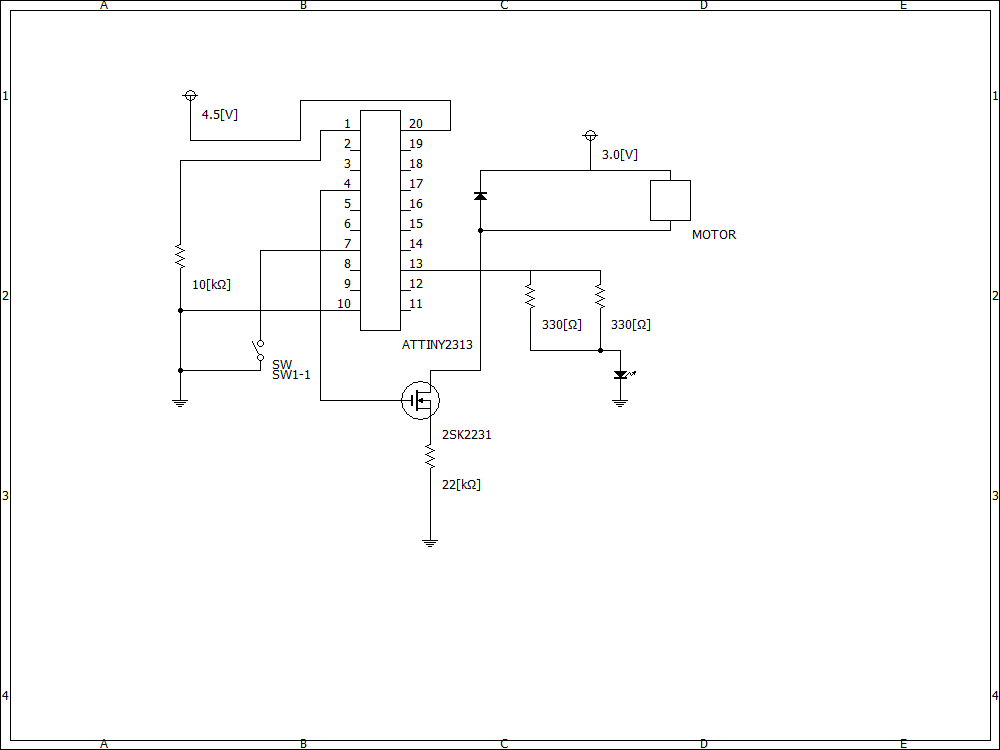
\includegraphics[width=15cm]{回路図.png}
 \end{center}
 \caption{回路図}
\end{figure}


\section{プログラムの説明}
今回使用したプログラムについて説明する。今回LEDをPORTBで制御し、またPORTDの2ピンをモータの制御、4ピンをスイッチからの電圧読み取りに使用している。また今回停止状態、高速状態、低速状態の遷移を制御する変数をstとして定義している。図2のような状態の遷移となる。またstに1が代入された時にモータとLEDを制御しその後stに2を代入し5秒数えている。また変数counterは5秒数えるための変数である。main関数にてled関数とmortor関数をwhile文にて実行しまたPORTD、PORTBの初期状態を設定している。led関数はLEDを制御、mortor関数はモータを制御また、停止状態、高速状態、低速状態のLEDの点滅時間をwaitStop、waitSm、waitFast、waitSlow関数で制御する。


\begin{figure}[htbp]
 \begin{center}
  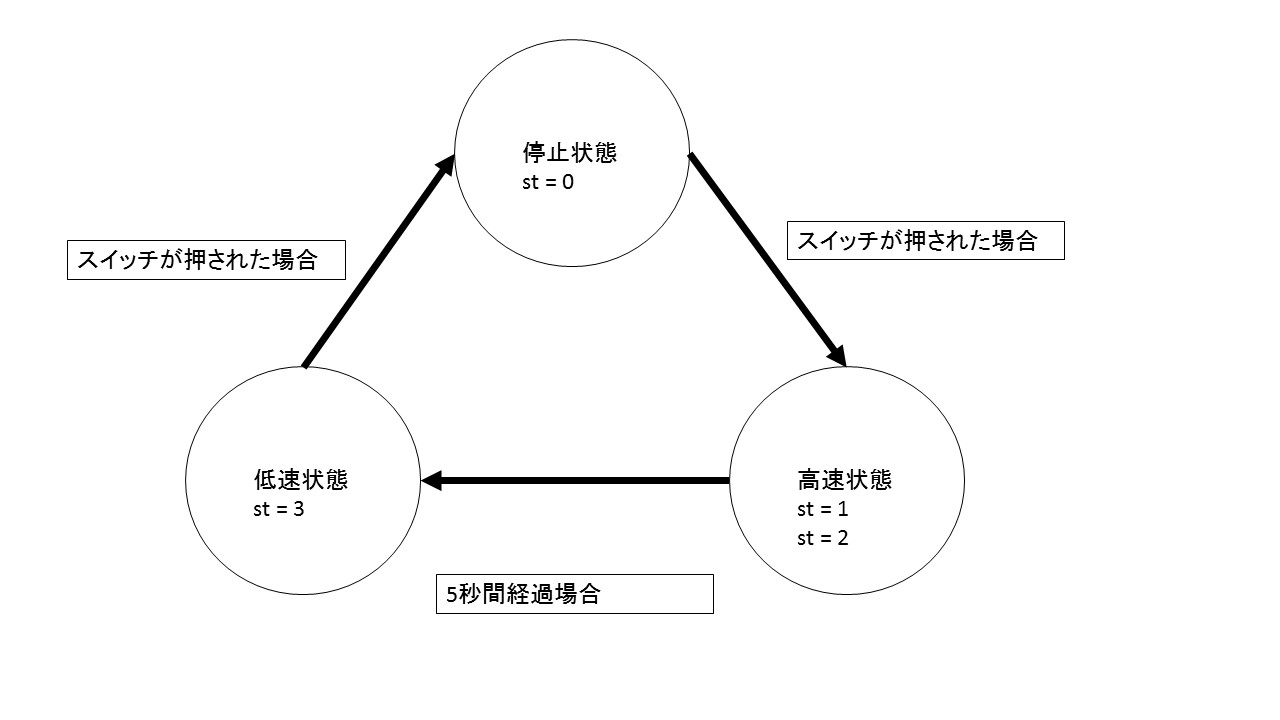
\includegraphics[width=15cm]{状態遷移図.jpg}
 \end{center}
 \caption{状態遷移図}
\end{figure}


\section{考察}
今回作成したコードでは長押ししなければ状態が遷移しないという事態が起きていたので改良する必要がある。また回路設計時にLEDに過大な電流が流れるように、マイコンにも負荷がかかるように回路を組んでしまっていた。今後FPGAボードなどの高額な機械を扱う場合に対して注意する必要があると考られる。また一番苦労した点としてはハードウェアプログラミング特有のプログラムの言語仕様であった。実際PORT指定に関しても正直なところ最初は理解が及んでいなかった。またc言語を今回利用したがint型の違いや、return文をmainに対して使用しないのは驚いた。最後に今回の課題を通して基本的なマイコンの扱いまた回路の設計に対する技術が向上したと考えられる。また自分はardinoのみしかマイコン関係を触れたことがなかったのでAVRマイコンに触れられたことは大変貴重な経験になったと思う。

\section{付録(プログラム)}
\begin{lstlisting}[basicstyle=\ttfamily\footnotesize, frame=single]
#include <avr/io.h>

int8_t st = 0;
int8_t counter = 0;
void led(void);
void mortor(void);
void waitSm(void);
void waitStop(void);
void waitFast(void);
void waitSlow(void);

int main(void){
	DDRB = 0xff;
	PORTB = 0xff;
	DDRD = 0xff;
	PORTD = 0;
	while(1){
		led();
		mortor();
	}
}


void led(void){
	switch(st){
		case 0:
		PORTB = 0xff;
		waitStop();
		PORTB = 0;
		waitStop();
		st = 0;
		while(PIND & (1<<4)){	
		st = 1;
		}
		break;
		case 1:
		PORTB = 0xff;
		waitFast();
		PORTB = 0;
		waitFast();
		counter++;
		if (counter > 4)
		st++;
		break;
		case 2:
		case 3:
		PORTB = 0xff;
		waitSlow();
		PORTB = 0;
		waitSlow();
		break;
	}
}
void mortor(void){
	switch(st){
		case 0:
		break;
		case 1:
		PORTD = 0x02;
		break;
		case 2:
		if(PIND & (1<<4))
		st=0;
		counter=0;
		PORTD = 0;
		break;
	}
}


void waitSm(void){
	volatile int32_t i;
	for(i=0;i<1000;i++){
	}
}

void waitStop(void){
	volatile int32_t i;
	for(i=0;i<150000;i++){
	}
}
void waitFast(void){
	volatile int32_t i;
	for(i=0;i<15000;i++){
	}
}
void waitSlow(void){
	volatile int32_t i;
	for(i=0;i<30;i++){
		PORTD = 0xff;
		waitSm();
		PORTD = 0;
		waitSm();
		i++;
	}
}

 \end{lstlisting}
\end{document}